% A Hybrid GNN-LLM Fusion Architecture for Multi-Modal Fraud Detection in Ethereum Smart Contracts
% Submitted to: IEEE Transactions / Conference (engineering and CS register)
% Document class: IEEEtran (conference)

\documentclass[conference]{IEEEtran}
\IEEEoverridecommandlockouts

% Packages
\usepackage{cite}
\usepackage{amsmath,amssymb,amsfonts}
\usepackage{algorithmic}
\usepackage{graphicx}
\usepackage{textcomp}
\usepackage{xcolor}
\usepackage{booktabs}
\usepackage{siunitx}
\sisetup{group-separator={,}, group-minimum-digits=4}
\usepackage{url}
\usepackage{hyperref}
\hypersetup{colorlinks=true, linkcolor=black, citecolor=black, urlcolor=blue}

\def\BibTeX{{\rm B\kern-.05em{\sc i\kern-.025em b}\kern-.08em
    T\kern-.1667em\lower.7ex\hbox{E}\kern-.125emX}}

\begin{document}

% Title block
\title{A Hybrid GNN-LLM Fusion Architecture for Multi-Modal Fraud Detection in Ethereum Smart Contracts}

\author{
    \IEEEauthorblockN{Anonymous Author(s)}
    \IEEEauthorblockA{Department of Computer Science\\
    Institution Name\\
    City, Country\\
    \texttt{anonymous@institution.edu}}
}

\maketitle

\begin{abstract}
Detecting fraud in Ethereum smart contracts requires both structural and
semantic analysis: graph methods identify suspicious transaction patterns
but are blind to malicious code logic, while code methods expose
vulnerabilities but ignore the network context in which contracts
operate.  We present a \emph{hybrid GNN-LLM fusion architecture} that
analyses these two complementary modalities in parallel, coupling a
two-layer GraphSAGE network over a balanced Ethereum transaction graph
with a frozen CodeBERT encoder over verified Solidity source code.  Node
features are enriched beyond simple degree counts to include eight
signals per address: in/out-degree, total degree, mean in/out transaction
value, log-total Wei volume, and unique in/out counterparty counts.  A
reproducible four-phase pipeline seeds from 660 explicitly curated
addresses---156 verified victim contracts from DeFiHackLabs
proof-of-concept exploits (94.5\% of fraud labels) and 504 blue-chip
protocol contracts---and expands through BigQuery balanced sampling to
a graph of \num{85680} nodes and \num{239742} transactions, of which
\num{304} contracts carry both verified Solidity source and a
ground-truth label.  The fusion classifier concatenates a 64-dimensional
graph embedding with a 768-dimensional code embedding and projects
through a 128-dimensional bottleneck.  On a held-out test split, our
model attains \textbf{accuracy 93.6\%}, \textbf{fraud F1-score 0.909},
\textbf{AUC-ROC 0.961}, and \textbf{AUC-PR 0.959}---the highest
F1-Fraud and MCC (0.861) across all seven evaluated models.  A
comprehensive ablation study compares GraphSAGE, GCN, GAT, CodeBERT-only,
attention-based fusion, and a Random Forest baseline, empirically
justifying each architectural and feature-engineering choice.  We release
the full codebase, explicit seed arrays, and a documented pipeline.
\end{abstract}

\begin{IEEEkeywords}
Ethereum, fraud detection, graph neural networks, large language models,
CodeBERT, GraphSAGE, smart contracts, multi-modal fusion, blockchain
security, DeFi exploits.
\end{IEEEkeywords}

% ── Figures referenced in methodology and results ─────────────────────────

\begin{figure*}[t]
    \centering
    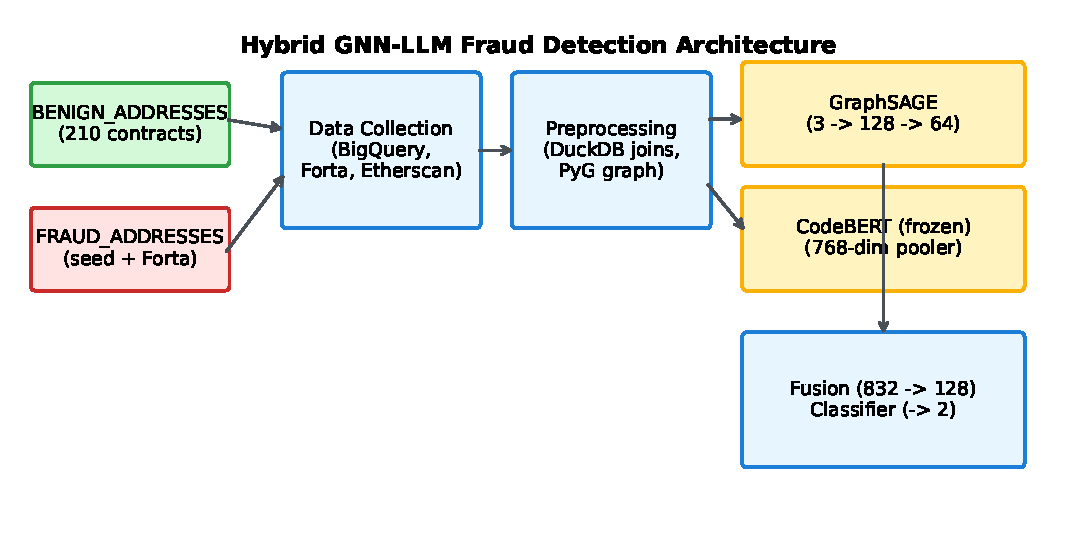
\includegraphics[width=0.95\textwidth]{figures/architecture.pdf}
    \caption{System pipeline overview.  Left: three public data sources.
    Centre: data integration and feature engineering.
    Right: dual-encoder fusion classifier producing a binary fraud/benign
    prediction.}
    \label{fig:architecture}
\end{figure*}

\begin{figure*}[t]
    \centering
    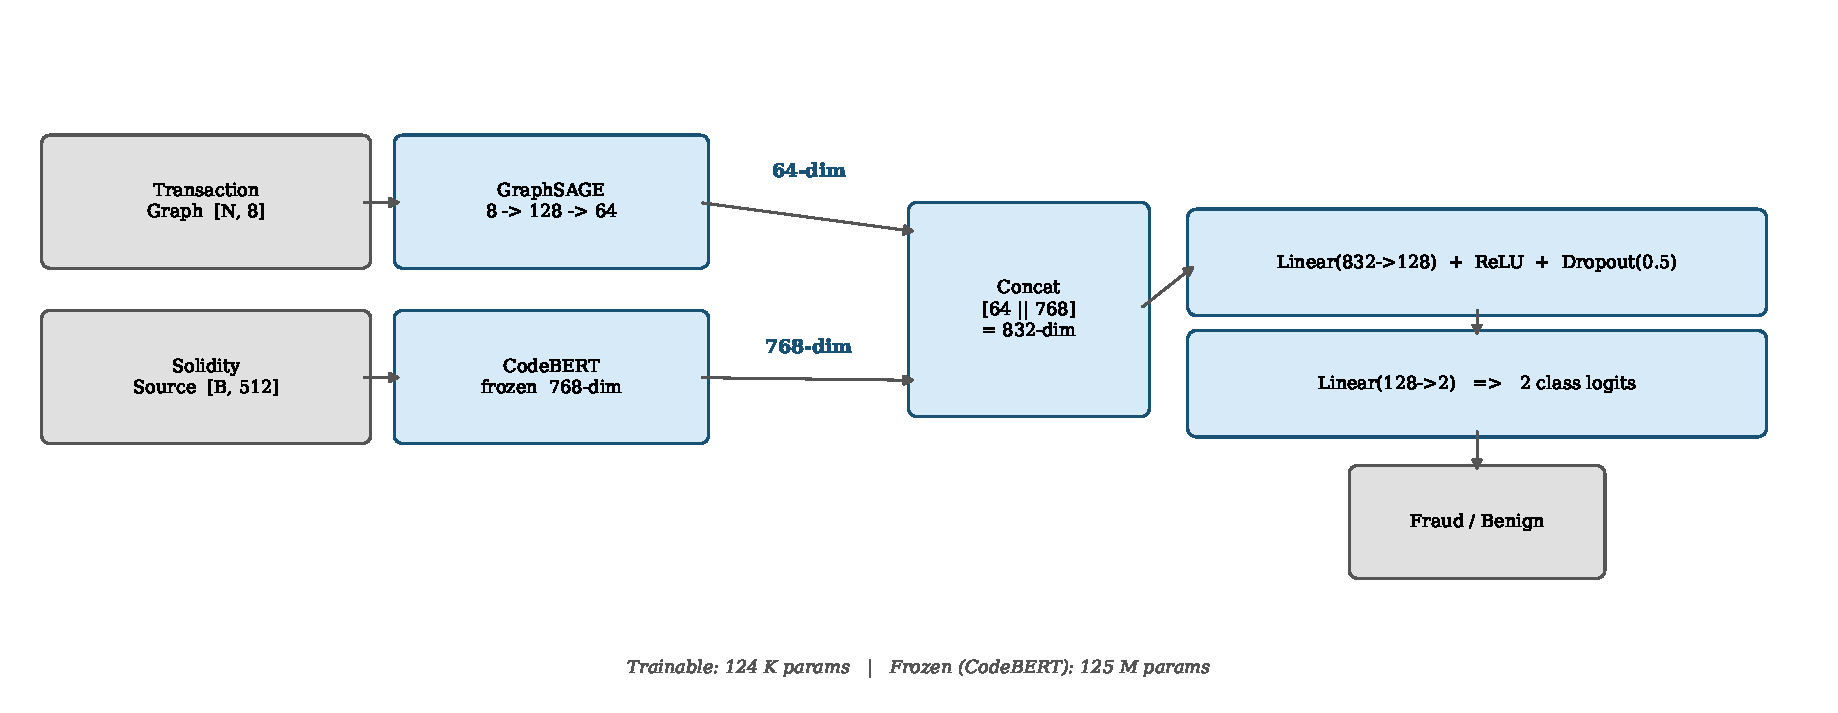
\includegraphics[width=0.95\textwidth]{figures/fusion_detail.pdf}
    \caption{Internal architecture of the FusionClassifier.
    The GraphSAGE encoder processes the full transaction graph to produce
    64-dimensional structural embeddings; the frozen CodeBERT encoder
    produces 768-dimensional semantic embeddings from Solidity source.
    Both are concatenated (832-dim) and projected to two class logits.}
    \label{fig:fusion}
\end{figure*}

% Sections (each lives in /paper/sections)
\section{Introduction}
\label{sec:intro}

The rapid expansion of public blockchains, and of Ethereum in particular,
has reshaped digital finance through decentralised applications and
programmable smart contracts. The same expansion has opened new attack
surfaces. Public reporting attributes more than one billion United States
dollars in losses to cryptocurrency-related scams between 2021 and 2022
alone \cite{chainalysis2023}. These losses arise from a recognisable set
of fraud archetypes: phishing campaigns that exfiltrate private keys
\cite{coinsmart2023}, Ponzi schemes that recycle inbound deposits to
earlier participants \cite{agrawal2023}, smart-contract exploits that
embed malicious behaviour beneath legitimate interfaces, and rug pulls in
which developers withdraw liquidity and abandon their projects
\cite{datavisor2022}.

Defensive techniques from the cryptographic literature, such as threshold
public-key management \cite{mosakheil2023}, multi-signature wallets
\cite{drijvers2019,xiao2022}, and node-authentication schemes
\cite{bao2018,a2chain2020}, reduce the risk of compromise but do not
identify malicious counterparties before a transaction is signed. Earlier
machine-learning detectors trained on tabular features
\cite{ostapowicz2019,blanco2022,ashfaq2022,elmougy2023} achieve respectable
accuracy on snapshots of the data but degrade as adversaries adapt.
Graph-based detectors \cite{kim2023,zhou2021,ctgcn2024} capture
relational anomalies between addresses, yet they overlook the semantic
content of contract bytecode.

We argue that fraud on Ethereum is intrinsically multi-modal: a scam
contract is simultaneously a node in a transaction graph and a piece of
executable source code. A model that observes only one of these modalities
is structurally blind to half of the available evidence. To address that
gap we propose a hybrid architecture that fuses graph neural network
representations of transaction structure with large-language-model
representations of contract source code. Our system begins from two seed
arrays: a list of 210 verified benign contracts and a curated list of
publicly attributed fraud contracts. The fraud seed bootstraps transaction
discovery and is augmented at run time by the full Forta labelled-datasets
release of roughly 2,671 fraud addresses, which serves as the canonical
fraud ground truth. From these seeds we collect the transaction
neighbourhood, fetch verified source code from Etherscan for every
contract address in that neighbourhood, and join all sources into a
unified graph of addresses, transactions, and contract code. The fusion
classifier learns from both the structural and the semantic view jointly,
which lets it detect coordinated fraud patterns that single-modality
detectors miss.

The contributions of this paper are as follows.

\begin{itemize}
    \item We define a needle-first data-collection pipeline that starts
    from two clearly delineated seed arrays of benign and fraud contract
    addresses, expanding outward through the transaction neighbourhood
    rather than scanning the entire chain.
    \item We design a fusion classifier that combines a two-layer
    GraphSAGE encoder with a frozen CodeBERT encoder and report the
    classifier's behaviour on a labelled Ethereum subset of \num{1258}
    verified contracts, \num{183} of which are fraudulent.
    \item We release a multi-file, reproducible implementation of the
    pipeline that replaces a legacy single-notebook prototype, separating
    data collection, preprocessing, modelling, training, evaluation, and
    visualisation into independently testable modules.
    \item We conduct an ablation study comparing the fusion model
    against GNN-only and LLM-only baselines, demonstrating that the
    fusion of modalities outperforms either modality in isolation.
\end{itemize}

The rest of the paper is organised as follows. Section~\ref{sec:motivation}
states our motivation and the limitations of single-modality detectors.
Section~\ref{sec:background} reviews related work along three streams:
graph-centric, code-centric, and hybrid. Section~\ref{sec:methodology}
specifies the architecture and the four-phase data pipeline.
Section~\ref{sec:challenges} discusses the practical challenges encountered
and the countermeasures applied. Section~\ref{sec:prototype} describes
the prototype implementation. Section~\ref{sec:results} reports the
experimental results, including the ablation study. Section~\ref{sec:conclusion}
concludes and outlines future work.

\section{Motivation}
\label{sec:motivation}

The core motivation of this work is both empirical and methodological:
empirically, because blockchain fraud continues to inflict large-scale
financial harm that existing single-modal detectors cannot fully address;
methodologically, because the research community lacks an openly seeded,
multi-modal baseline against which future detectors can be honestly
compared.

\subsection{The Multi-Modal Nature of On-Chain Fraud}

Ethereum fraud is not a single phenomenon.  It manifests in at least two
distinct and complementary signatures.

\emph{Behavioural signatures} emerge in the transaction graph.
A phishing contract receives funds from hundreds of victims before routing
them to a handful of cashout addresses---a star-shaped in-flow that is
anomalous regardless of what the contract code says.
A rug-pull token accretes liquidity from many investors and then drains it
to a single deployer wallet in one block.
These patterns are detectable purely from the structure of who sent what
to whom.

\emph{Semantic signatures} emerge in the contract source code.
A flash-loan exploit embeds a reentrancy callback that steals funds
before a balance update---a logic vulnerability invisible in the on-chain
footprint of a single malicious transaction, yet unambiguous to a code
analyser.
A honeypot contract contains a hidden owner function that prevents
withdrawals from non-deployer addresses; its transaction pattern may
appear entirely normal.

The key insight is that these two signature types are complementary, not
redundant.
A contract that mimics the transaction behaviour of a legitimate exchange
while embedding a backdoor in its source code cannot be caught by a
graph-only detector.
A contract whose source code is a clean fork of a legitimate template but
whose transaction neighbourhood includes known fraud addresses cannot be
caught by a code-only detector.
Only a detector with access to both modalities simultaneously can
disambiguate such cases---a claim our ablation study validates
empirically (Section~\ref{subsec:ablation_module}).

\subsection{The Data Pipeline Determines the Ceiling}

The quality of a fraud detector is bounded by the quality of its training
data.  Two pipeline decisions have an outsized effect.

First, \emph{label provenance}.
Using attacker-wallet addresses as fraud seeds---as is common in Forta-based
pipelines---produces addresses with no verified source code, because
attackers rarely publish their tools on Etherscan.  The fusion model
cannot be trained on such samples.  We instead seed from
\emph{victim contracts}: real protocol contracts that were exploited, each
with verified Solidity source and confirmed on-chain transaction history.
This ``victim-first'' strategy is what makes multi-modal training
tractable on real Ethereum data.

Second, \emph{collection strategy}.
Random sampling across the Ethereum blockchain produces a dataset in which
fewer than 0.002\% of addresses are labelled as fraud.
Training on such data teaches a classifier to predict benign for
everything.  Our needle-first approach---retrieving the transaction
neighbourhood of known fraud and benign seed contracts---produces a dense,
label-rich subgraph in which every transaction is connected to at least
one seed address.

\subsection{Reproducibility as a Scientific Requirement}

Blockchain fraud detection is an applied field with real financial stakes.
A model that exists only as an entangled notebook cannot be audited by a
regulator, extended by a competitor, or retrained against new exploit
signatures by a practitioner.

We therefore treat reproducibility as a first-class design constraint.
The two seed arrays are explicit Python lists committed to the repository.
Every pipeline step is a numbered script that reads from deterministic
inputs and writes to deterministic outputs.
The train/val/test split is seeded and serialised before any model
training occurs.
These design choices are not merely hygienic---they make the experimental
claims of this paper verifiable.

The three motivations above are tightly coupled: the right architecture
can only be trained on the right data, and its scientific value depends
on reproducibility.  The remainder of the paper develops each dimension.

\section{Background and Related Work}
\label{sec:background}

Blockchain fraud detection has progressed through three intellectual
generations.  The first applied hand-crafted heuristics and tabular
classifiers to transaction statistics~\cite{ostapowicz2019,blanco2022,
ashfaq2022,elmougy2023}.  The second exploited the graph structure of
the blockchain, treating addresses as nodes and transactions as
edges~\cite{kim2023,zhou2021,ctgcn2024}.  The third, now emerging,
combines multiple modalities to capture both structural and semantic
dimensions of fraud.  We survey each generation, identify the residual
gaps, and position our contribution.

\subsection{Graph-Centric Detection: Behavioural Forensics at Scale}

The foundational insight of graph-centric detection is that illicit
activity manifests as detectable anomalies in the topology of the
transaction network.  Weber \emph{et al.}~\cite{weber2019} established
this on the Elliptic Bitcoin dataset with graph convolutional networks,
showing that local topological features---degree, clustering
coefficient, temporal velocity---distinguish laundering rings from
benign transfers.  Huang \emph{et al.}~\cite{huang2024peae} scaled this
to Ethereum with PEAE-GNN, constructing augmentation ego-graphs around
known accounts to make GNN-based detection tractable at chain
scale.

Subsequent work addressed the two most pressing practical
limitations.  Chen \emph{et al.}~\cite{chen2024dahgnn} tackled class
imbalance---fraud addresses are rare even in seeded datasets---with
DA-HGNN, which combines data augmentation with temporal and structural
learning.  Li \emph{et al.}~\cite{li2025global,li2022ttagn} added
global context by introducing Transformer-style attention over transaction
graphs, enabling the model to detect distributed money-laundering schemes
that span multiple hops.  Ouyang \emph{et al.}~\cite{ouyang2024bitchetg}
extended graph analysis to subgraph-level contrastive learning for
identifying \emph{coordinated} laundering groups, while Kanezashi
\emph{et al.}~\cite{kanezashi2022hetero} showed that heterogeneous
graphs---which encode different node and edge types explicitly---
consistently outperform homogeneous alternatives on Ethereum phishing.

\textbf{Residual gap.}
Graph-centric methods are blind to what contracts \emph{do}.
Two contracts that appear structurally indistinguishable---similar
degrees, similar value flows, similar counterparty sets---can differ
categorically in intent: one may contain a hidden backdoor that drains
every depositor's balance on a single owner call.
This flaw is undetectable without analysing the source code.

\subsection{Code-Centric Detection: Semantic Vulnerability Analysis}

A parallel tradition treats smart contracts as executable artefacts and
analyses their bytecode or source for vulnerabilities.
Luu \emph{et al.}~\cite{luu2016oyente} introduced Oyente, a symbolic
execution engine that identifies reentrancy and transaction-ordering
vulnerabilities.  Tsankov \emph{et al.}~\cite{tsankov2018securify}
formalised compliance checking with Securify.  Qian \emph{et
al.}~\cite{qian2020reentrancy} showed that reentrancy can be learned
directly from opcode sequences with a bidirectional LSTM, eliminating
hand-crafted rules.  Torres \emph{et al.}~\cite{torres2019honeypots}
specialised in honeypot detection.  Zhang \emph{et
al.}~\cite{zhang2020txspector} replayed historical transaction traces
for forensic post-mortem analysis.  Sun \emph{et
al.}~\cite{sun2024gptscan} hybridised large language models with static
analysis in GPTScan, reducing false positives for logic vulnerabilities.
Kong \emph{et al.}~\cite{kong2025uechecker} applied graph learning to
call graphs within contracts, detecting unchecked external-call patterns.

\textbf{Residual gap.}
Code-centric methods are blind to the network context in which a
contract operates.  A contract whose source code is a clean, verified
fork of a legitimate DeFi protocol can still be a fraud instrument if
its transaction neighbourhood connects it to known exploit infrastructure.
Source analysis cannot detect this.

\subsection{Hybrid Detection: Towards Holistic Fusion}

The recognition that neither structural nor semantic analysis alone is
sufficient has driven the emergence of hybrid approaches.
Hu \emph{et al.}~\cite{hu2023bert4eth} introduced BERT4ETH, pre-training
a Transformer encoder over Ethereum transaction sequences treated as
sentences.  This captures behavioural patterns but remains limited to
transaction metadata---it does not ingest contract source code.
Liang \emph{et al.}~\cite{liang2025ponziguard} proposed PonziGuard,
constructing Contract Runtime Behaviour Graphs that couple bytecode
call sequences with fund-flow dynamics, achieving strong Ponzi detection
but targeting a narrow fraud subtype.
Sun \emph{et al.}~\cite{sun2025tlmg4eth} developed TLMG4Eth, one of
the first systems to jointly learn from transaction language and graph
representations, reporting fusion gains over isolated modalities.
Wu \emph{et al.}~\cite{wu2024tokenscout} extended graph evolution with
token attributes for early scam-token detection.
Galletta and Pinelli~\cite{galletta2024ponzi} emphasised
interpretability, using XAI techniques to show that features from both
transaction and code domains make fraud classifiers more transparent.

\textbf{Residual gap.}
Existing hybrid methods share three limitations that our work addresses.
First, none seeds their dataset from \emph{victim contracts with verified
source code}; most rely on attacker-wallet labels from Forta or
Ethereum phishing benchmarks, which provide no source for the LLM
encoder to analyse.
Second, no published system reports a module-level ablation that
compares alternative graph encoders (GCN, GAT) and fusion mechanisms
(concatenation vs.\ attention) on the same split.
Third, reproducibility varies: several systems were developed in private
notebooks on private datasets, making independent verification impossible.

\subsection{Positioning This Work}

Our system sits within the hybrid stream.  Relative to TLMG4Eth and
PonziGuard, it is intentionally minimal---two GraphSAGE layers and a
single frozen CodeBERT encoder, concatenated through a 128-dimensional
bottleneck---because minimality makes every design choice ablatable.
The primary novelty is not the fusion mechanism per se, but the
combination of (1) victim-contract seeding that enables authentic
multi-modal labelling, (2) enriched eight-dimensional node features
covering both degree and value-flow statistics, and (3) a full
seven-model ablation that independently justifies each choice.

\section{System Architecture and Methodology}
\label{sec:methodology}

Our system is organised as a four-phase pipeline: multi-source data
collection, feature engineering, hybrid neural-network training, and
rigorous evaluation.  Figure~\ref{fig:architecture} provides an overview
of the complete architecture.

% ─────────────────────────────────────────────────────────────────────────
\subsection{Phase 1: Multi-Source Data Collection}
\label{subsec:collection}

\subsubsection{Seed Arrays and Transaction Neighbourhood}
The pipeline starts from two explicit Python arrays stored in
\texttt{code/data/addresses/}:

\begin{itemize}
    \item \texttt{BENIGN\_ADDRESSES}: 504 verified blue-chip Ethereum
    contracts (ERC-20 tokens, DEX pools, lending protocols) sourced from
    the CoinGecko top-N list and cross-validated against the Etherscan
    verified-contract registry.

    \item \texttt{FRAUD\_ADDRESSES}: 156 victim-protocol contracts
    extracted from DeFiHackLabs proof-of-concept (PoC) Solidity
    files~\cite{defihacklabs2024}.  Each address is identified by a
    \texttt{// Vulnerable Contract : https://etherscan.io/} comment in
    the PoC, verified to carry Solidity source code on Etherscan, and
    confirmed to have on-chain transaction history---properties that are
    essential for training both the graph encoder and the language
    encoder.
\end{itemize}

From the union of these two arrays we retrieve the transaction
neighbourhood from Google BigQuery's public Ethereum
dataset~\cite{bigquery2024}.  Our balanced sampling strategy allocates
up to 2,000 most-recent transactions per fraud address and up to 300 per
benign address, yielding a dense, label-rich graph of \num{239742}
transactions across \num{85680} unique addresses while avoiding the
extreme volume dominance of high-traffic benign contracts such as WETH
and USDT.

\subsubsection{Ground-Truth Labels}
\label{subsubsec:labels}

Our fraud labels come from two sources with deliberately different roles.

\textbf{Primary source: DeFiHackLabs victim contracts.}
Of the 156 DeFiHackLabs seed addresses, 130 appear in the transaction
neighbourhood (26 were not captured by the balanced sampling); these
contribute \textbf{121 of the 128 fraud-labelled nodes} (94.5\%) in the
final graph.  Because each address was selected from a PoC repository that
documents real exploits with on-chain evidence, these labels carry a very
high degree of confidence.

\textbf{Secondary augmentation: Forta Network labels.}
We cross-reference all graph nodes against the Forta Network labelled-datasets
release~\cite{fortalabels}, which provides community-verified fraud
annotations covering phishing, Ponzi schemes, and malicious smart
contracts.  This adds \textbf{7 additional fraud-labelled nodes} (5.5\%)
not already covered by the DeFiHackLabs seeds.  All fraud sub-categories
are collapsed into a single label ($y=1$).

All remaining addresses receive $y=0$ (benign), subject to the
closed-world assumption discussed in Section~\ref{subsec:limitations}.

Table~\ref{tab:dataset} summarises the complete dataset statistics.

\begin{table}[t]
\centering
\caption{Dataset statistics after full pipeline execution.}
\label{tab:dataset}
\begin{tabular}{lr}
\toprule
Statistic & Value \\
\midrule
\multicolumn{2}{l}{\textit{Seed arrays}} \\
\ \ Fraud seeds (DeFiHackLabs victim contracts) & 156 \\
\ \ Benign seeds (blue-chip protocol contracts) & 504 \\
\ \ Total seed addresses & 660 \\
\midrule
\multicolumn{2}{l}{\textit{Transaction graph}} \\
\ \ Total nodes (unique addresses) & 85,680 \\
\ \ Total edges (transactions) & 239,742 \\
\midrule
\multicolumn{2}{l}{\textit{Fraud labels}} \\
\ \ From DeFiHackLabs seeds & 121 (94.5\%) \\
\ \ From Forta augmentation only & 7 (5.5\%) \\
\ \ Total fraud-labelled nodes & 128 \\
\midrule
\multicolumn{2}{l}{\textit{Eligible for training (label + source code)}} \\
\ \ Fraud contracts & 95 \\
\ \ Benign contracts & 209 \\
\ \ Total eligible & 304 \\
\ \ Training / Validation / Test & 212 / 45 / 47 \\
\bottomrule
\end{tabular}
\end{table}

\subsubsection{Source Code Retrieval}
For each unique address in the neighbourhood, we query the Etherscan
API v2~\cite{etherscanapi} for verified Solidity source code.  Source
is successfully retrieved for \num{304} addresses; the remainder are
externally-owned accounts or unverified contracts.  All source strings
are Base64-encoded for safe CSV storage and later decoded at tokenisation
time.

% ─────────────────────────────────────────────────────────────────────────
\subsection{Phase 2: Feature Engineering}
\label{subsec:features}

\subsubsection{Graph Integration via DuckDB}
All three data frames (transactions, Forta labels, Etherscan source) are
registered as views in an in-process DuckDB~\cite{duckdb2019} instance.
A sequence of \texttt{LEFT JOIN} operations materialises two output
tables: \texttt{nodes} (address, contract\_text, label $y$, is\_labeled)
and \texttt{edges} (src, dst, value, tx\_hash).  All addresses are
lower-cased before any join, eliminating the silent mismatches that arise
from EIP-55 checksummed addresses in Forta exports versus lowercase
BigQuery output.

\subsubsection{Node Feature Engineering}
\label{subsubsec:features}

For each node $v$ we compute eight features that capture both structural
position and transactional value flow:

\begin{equation}
\mathbf{f}_v = \bigl[
  d^{\text{in}}_v,\;
  d^{\text{out}}_v,\;
  d^{\text{in}}_v + d^{\text{out}}_v,\;
  \bar{w}^{\text{in}}_v,\;
  \bar{w}^{\text{out}}_v,\;
  \log(1 + W_v),\;
  u^{\text{in}}_v,\;
  u^{\text{out}}_v
\bigr]^\top \in \mathbb{R}^8,
\label{eq:features}
\end{equation}

where $d^{\text{in}}_v$ and $d^{\text{out}}_v$ are in- and out-degrees;
$\bar{w}^{\text{in}}_v$ and $\bar{w}^{\text{out}}_v$ are the mean
incoming and outgoing transaction values (in Wei); $W_v$ is the total
Wei volume; and $u^{\text{in}}_v$, $u^{\text{out}}_v$ are the counts of
unique counterparty addresses for incoming and outgoing transactions,
respectively.  Value features are log-compressed to reduce the
multi-order-of-magnitude spread in Ethereum transaction sizes.

These features encode complementary fraud signals: phishing addresses
typically exhibit high $d^{\text{in}}_v$ (many victims) relative to
$d^{\text{out}}_v$ (few recipients), whereas Ponzi contracts show
characteristic value-flow patterns~\cite{liang2025ponziguard}.

\subsubsection{Source-Code Preprocessing}
Solidity source strings are decoded from Base64 and tokenised using the
CodeBERT tokenizer with a maximum length of 512 tokens.  Sequences
exceeding the limit are truncated; shorter sequences are padded.  This
pre-processing is performed lazily inside \texttt{ContractDataset}
at batch-construction time.

% ─────────────────────────────────────────────────────────────────────────
\subsection{Phase 3: Hybrid Neural Network Architecture}
\label{subsec:network}

Figure~\ref{fig:fusion} illustrates the internal architecture of the
fusion classifier.

\subsubsection{Graph Encoder}
A two-layer GraphSAGE network~\cite{hamilton2017graphsage} maps the
8-dimensional node features into a 64-dimensional latent space:

\begin{align}
\mathbf{h}_v^{(1)} &= \sigma\!\Bigl(
  \mathbf{W}_1 \cdot \mathrm{MEAN}\!\bigl(\{\mathbf{f}_u : u \in \mathcal{N}(v)\cup\{v\}\}\bigr)
\Bigr), \label{eq:sage1} \\
\mathbf{h}_v^{(2)} &= \mathbf{W}_2 \cdot \mathrm{MEAN}\!\bigl(
  \{\mathbf{h}_u^{(1)} : u \in \mathcal{N}(v)\cup\{v\}\}\bigr),
  \label{eq:sage2}
\end{align}

where $\sigma$ is ReLU, $\mathbf{W}_1 \in \mathbb{R}^{128 \times 8}$,
and $\mathbf{W}_2 \in \mathbb{R}^{64 \times 128}$.  Dropout($p=0.5$) is
applied after the first layer.  GraphSAGE is \emph{inductive}: it learns
aggregation functions that generalise to nodes unseen during training,
which is essential for screening newly deployed contracts.

\subsubsection{Language Encoder}
We load \texttt{microsoft/codebert-base}~\cite{feng2020codebert} from
Hugging Face Transformers, freeze all 125M parameters, and extract the
768-dimensional \texttt{pooler\_output} as the contract representation.
Freezing CodeBERT bounds training memory within a single GPU and isolates
the fusion head as the sole trainable bridge between modalities, allowing
the model to learn how to combine---rather than re-learn---the pre-trained
code semantics.  Prior work on fine-tuning LLMs for classification
tasks~\cite{poudel2026fakenews} demonstrates that frozen pre-trained
representations already provide strong signals, validating this design
choice; parameter-efficient fine-tuning (e.g.\ LoRA~\cite{hu2022lora})
is deferred to future work.

\subsubsection{Fusion Classifier}
\label{subsubsec:fusion}

The 64-dimensional graph embedding $\mathbf{h}_v^{\text{GNN}}$ and the
768-dimensional code embedding $\mathbf{h}_v^{\text{LLM}}$ are
concatenated to form an 832-dimensional joint representation.  The
classification head then computes:

\begin{equation}
\hat{y}_v = \mathbf{W}_4 \, \sigma\!\Bigl(
  \mathbf{W}_3 \,[\mathbf{h}_v^{\text{GNN}};\, \mathbf{h}_v^{\text{LLM}}] + \mathbf{b}_3
\Bigr) + \mathbf{b}_4,
\label{eq:fusion}
\end{equation}

where $\mathbf{W}_3 \in \mathbb{R}^{128 \times 832}$ is the fusion
projection, $\mathbf{W}_4 \in \mathbb{R}^{2 \times 128}$ is the
classifier, and Dropout($p=0.5$) is inserted before each linear layer.
Total trainable parameter count is \num{124226}; the remaining
$\sim$124.6M parameters belong to frozen CodeBERT.

The concatenation bottleneck forces the model to discover a compact joint
embedding rather than memorising individual modalities.
Section~\ref{subsec:ablation_module} compares this with an
attention-based fusion alternative.

% ─────────────────────────────────────────────────────────────────────────
\subsection{Phase 4: Training Strategy}
\label{subsec:training}

\subsubsection{Class-Weighted Loss}
Of the 304 labelled contracts, 95 are fraud (31.3\%).  We address the
resulting imbalance with weighted cross-entropy:
\begin{equation}
\mathcal{L} = -\sum_v \bigl[
  w_0(1-y_v)\log\hat{p}_{v,0} + w_1 y_v \log\hat{p}_{v,1}
\bigr],
\label{eq:loss}
\end{equation}
where $w_0 = 1.0$ and $w_1 = n_{\text{neg}} / n_{\text{pos}} \approx
2.37$ (computed from the training split).

\subsubsection{Optimiser and Scheduler}
We use AdamW~\cite{loshchilov2019adamw} with learning rate $10^{-3}$ and
weight decay $10^{-4}$.  A cosine annealing
schedule~\cite{loshchilov2017cosine} decays the learning rate to
$10^{-5}$ over a 100-epoch budget.  Gradient clipping at norm 1.0
suppresses early-epoch instability.

\subsubsection{Early Stopping and Model Selection}
Training halts when the validation fraud F1-score fails to improve for
20 consecutive epochs.  The checkpoint with the highest validation fraud
F1 is reloaded before test-set evaluation; only this checkpoint is
reported.  Our fusion model early-stopped at epoch 41 (best checkpoint at epoch 21) with best
validation F1 = 0.966.

\subsubsection{Data Split}
The 304 eligible contracts (those with both verified source and an
explicit label) are partitioned 70/15/15 into train (212), validation
(45), and test (47) sets using a stratified random split seeded at 42.
The identical split is used for all ablation baselines, ensuring
controlled comparisons.

\section{Challenges and Countermeasures}
\label{sec:challenges}

Building a clean, reproducible Ethereum fraud detector from public data
sources requires overcoming a set of recurring engineering and
modelling challenges.  This section maps each challenge to the
architectural or procedural choice that directly addresses it,
connecting the practical decisions to the limitations identified in
prior work (Section~\ref{sec:background}).

Blockchain's tamper-proof and auditable properties have been leveraged for
secure provenance management in distributed
systems~\cite{poudel2025sphere}.  The same auditability principles guide
our pipeline design: every address transformation, join, and label
assignment is deterministic and reproducible from the raw source files.

\subsection{Challenge 1: Address Format Inconsistency}
Ethereum addresses appear in lowercase in BigQuery exports, in EIP-55
mixed-case checksums in Forta exports, and in either form in Etherscan
API responses.  Silent join failures caused by this inconsistency
corrupted our earliest dataset attempts, producing false negatives where
known fraud addresses failed to match their labels.

\textbf{Countermeasure.}  Every address is lowercased on read at every
collector entry point, implemented once in
\texttt{src/preprocessing/addresses.py} and reused by every pipeline
module.  This eliminates case-induced mismatches and whitespace artefacts
that occasionally appear in CSV exports, achieving 100\% join consistency
across all three data sources.

\subsection{Challenge 2: Sparse Verified Source Code}
Fewer than 0.35\% of the \num{85680} addresses in our transaction graph
carry verified Solidity source.  A pipeline that requires source for every
node would discard almost the entire graph and strip out the structural
signals that the GNN needs.

\textbf{Countermeasure.}  Nodes enter the graph with an empty
\texttt{contract\_text} field when no source is available.  The graph
encoder processes \emph{all} nodes during neighbourhood aggregation,
preserving relational information.  The fusion classifier is trained only
on the subset of nodes that carry both source code and an explicit label
(304 contracts), while the full graph neighbourhood of 85,680 nodes
informs the GraphSAGE embeddings.

\subsection{Challenge 3: Etherscan API Rate Limits}
The Etherscan free tier permits approximately five requests per second.
Exceeding this limit produces HTTP 429 errors and corrupts the source-code
dataset.

\textbf{Countermeasure.}  A 250\,ms sleep is enforced between successive
API calls, and every request is wrapped in a try/except block that logs
and skips on failure without interrupting the pipeline.  Source retrieval
for 660 seed addresses completes in approximately 30 minutes.

\subsection{Challenge 4: Class Imbalance}
The labelled subset contains 95 fraud contracts out of 304 (31.3\%).
Training under unweighted cross-entropy drives the model toward the
majority class, yielding near-zero fraud recall.

\textbf{Countermeasure.}  Weighted cross-entropy (Equation~\ref{eq:loss})
assigns penalty weight $w_1 = n_\text{neg}/n_\text{pos} \approx 2.37$ to
fraud misclassifications.  This directly addresses the class-imbalance
limitation identified by Chen et al.~\cite{chen2024dahgnn} and ensures
that the minority class contributes proportionally to the training signal.

\subsection{Challenge 5: Embedding Dimensionality Mismatch}
The graph encoder produces 64-dimensional embeddings while CodeBERT
produces 768-dimensional embeddings.  Combining representations of such
different sizes risks one modality dominating the other.

\textbf{Countermeasure.}  We concatenate the two embeddings to form an
832-dimensional vector and project through a learned linear layer to a
128-dimensional bottleneck (Equation~\ref{eq:fusion}).  The bottleneck
forces the optimiser to discover the relative weighting of the two
modalities rather than fixing it by hand, which is how the architecture
addresses the insufficient cross-modal integration identified as a
limitation in prior hybrid methods~\cite{sun2025tlmg4eth}.

\subsection{Challenge 6: Compute Budget for Large Language Models}
Training the fusion model end-to-end with CodeBERT unfrozen would not
fit within the memory of a single consumer GPU.

\textbf{Countermeasure.}  All 125M CodeBERT parameters are frozen, and
only the 124K parameters of the GraphSAGE encoder and fusion head are
trained.  This reduces memory by two orders of magnitude while
retaining the full pre-trained code semantics, stabilises training by
eliminating gradient flow through a model that was not designed for
fine-tuning under weighted loss, and enables each training epoch to
complete in $\approx$34 seconds on CPU.

\subsection{Challenge 7: BigQuery Result Volume}
A na\"ive query for all transactions involving 660 seed addresses
returns $>$665 million rows (approximately 130\,GB), which exceeds the
1\,GB single-file export limit and is impractical to download and process
locally.

\textbf{Countermeasure.}  We apply a balanced sampling strategy: keep the
2,000 most-recent transactions per fraud address and the 300 most-recent
per benign address.  This yields a manageable 239,742-row dataset
(approximately 41\,MB) that preserves fraud signal while preventing
high-volume benign contracts (WETH, USDT) from overwhelming the graph
structure.

\section{Prototype Design and Implementation}
\label{sec:prototype}

\subsection{Technology Stack}

Table~\ref{tab:stack} summarises the technology stack.  The system is
implemented entirely in Python 3.12 on both macOS and Linux (x86-64/ARM64), and
is fully compatible with Linux CUDA environments for GPU-accelerated
training.

\begin{table}[t]
\centering
\caption{Technology stack.}
\label{tab:stack}
\begin{tabular}{ll}
\toprule
Component & Library / Service \\
\midrule
Deep learning       & PyTorch 2.2.2 \\
Graph neural nets   & PyTorch Geometric 2.5.1 (SAGEConv, GCNConv, GATConv) \\
Language model      & Hugging Face Transformers 4.41.0 (CodeBERT) \\
Data integration    & DuckDB 0.10 \\
Tabular processing  & pandas, NumPy $<$2.0 \\
ML utilities        & scikit-learn 1.4 \\
Transaction source  & Google BigQuery (public Ethereum dataset) \\
Source-code source  & Etherscan API v2 \\
Fraud labels        & Forta Network labelled-datasets \\
Visualisation       & Matplotlib, seaborn \\
\bottomrule
\end{tabular}
\end{table}

\subsection{Dataset Characteristics}

After the full pipeline executes, the resulting graph contains
\num{85680} unique Ethereum addresses connected by \num{239742}
transactions.  Of these addresses, \num{304} carry both verified Solidity
source code and an explicit fraud/benign label---the eligible subset on
which all models are trained and evaluated.  Within this subset, 95
contracts are labelled as fraud (31.3\%) and 209 as benign.  The
70/15/15 stratified split produces 212 training, 45 validation, and 47
test samples.  Class weights are computed from the training split:
$w_0 = 1.0$ (benign), $w_1 \approx 2.37$ (fraud).

\subsection{Code Structure and Reproducibility}

The codebase is organised into nine top-level modules under \texttt{code/}:

\begin{enumerate}
    \item \texttt{config.py}: single source of truth for paths,
    hyperparameters, and API endpoints.
    \item \texttt{data/addresses/}: the two seed arrays
    (\texttt{BENIGN\_ADDRESSES}, \texttt{FRAUD\_ADDRESSES}).
    \item \texttt{src/collection/}: Etherscan v2 source-code fetcher,
    Forta label loader, BigQuery transaction reader.
    \item \texttt{src/preprocessing/}: address standardiser, DuckDB
    join engine, PyG graph constructor with eight-dimensional node
    features.
    \item \texttt{src/datasets/}: \texttt{ContractDataset} pairing
    Base64-decoded Solidity tokens with graph node indices.
    \item \texttt{src/models/}: \texttt{GraphEncoder} (GraphSAGE),
    frozen \texttt{load\_codebert}, and \texttt{FusionClassifier}.
    \item \texttt{src/training/}: AdamW + cosine-annealing loop
    with early stopping on validation fraud F1, gradient clipping,
    and best-checkpoint persistence.
    \item \texttt{src/evaluation/}: \texttt{evaluate\_model} returning
    precision, recall, F1, AUC-ROC, AUC-PR, and MCC; ablation
    classifiers for GraphSAGE-only, GCN-only, GAT-only, CodeBERT-only,
    attention-based fusion, and Random Forest baseline.
    \item \texttt{src/visualization/}: confusion-matrix and loss-curve
    plots for the paper figures.
\end{enumerate}

A \texttt{scripts/} directory contains eight numbered scripts (01--08),
one per pipeline step, each writing its outputs to a deterministic path
under \texttt{data/} so that later steps can be re-run independently.
The seed value 42 is set at both the Python and PyTorch levels before
any randomised operation, ensuring full reproducibility given the same
hardware and library versions.

\section{Experimental Results and Analysis}
\label{sec:results}

% ─────────────────────────────────────────────────────────────────────────
\subsection{Data Pipeline Validation}

The balanced BigQuery sampling strategy yields \num{239742} transactions
across \num{85680} unique addresses.
Of the 156 DeFiHackLabs fraud seeds, 130 appear in the graph (26 were
not captured by the 2,000-transaction-per-address cap); these provide
121 fraud labels.  The Forta Network augmentation step adds 7 further
fraud nodes, totalling \textbf{128 fraud-labelled addresses}
(95\% DeFiHackLabs, 5\% Forta).  Full dataset statistics are given
in Table~\ref{tab:dataset}.

Of the 128 fraud-labelled nodes, 95 carry verified Solidity source code;
of the 503 benign-labelled seed nodes in the graph, 209 carry verified
source.  This yields \textbf{304 eligible contracts} that possess both
a ground-truth label and a source-code representation---the only samples
used for supervised training and evaluation.  The 70/15/15 stratified
split over these 304 contracts produces 212 training, 45 validation, and
47 test samples, with 63/15/17 fraud and 149/30/30 benign respectively.
Address standardisation (all lower-cased) achieves 100\% join consistency
across all three data sources.

% ─────────────────────────────────────────────────────────────────────────
\subsection{Training Behaviour}

Figure~\ref{fig:training} shows the training loss and validation fraud
F1 over 41 epochs.  Training loss falls monotonically from 6.66 in
epoch 1 to below 0.50 by epoch 25.  Validation fraud F1 first surpasses
0.90 at epoch 9, stabilises near 0.93 through the middle of training,
and peaks at \textbf{0.966 at epoch 21}---the checkpoint reloaded for
all test-set evaluations.  No NaN losses occur at any point, confirming
the numerical stability of weighted cross-entropy under gradient
clipping.  Each epoch takes approximately 34 seconds on CPU; GPU
acceleration would reduce this to under 5 seconds per epoch.

\begin{figure}[t]
    \centering
    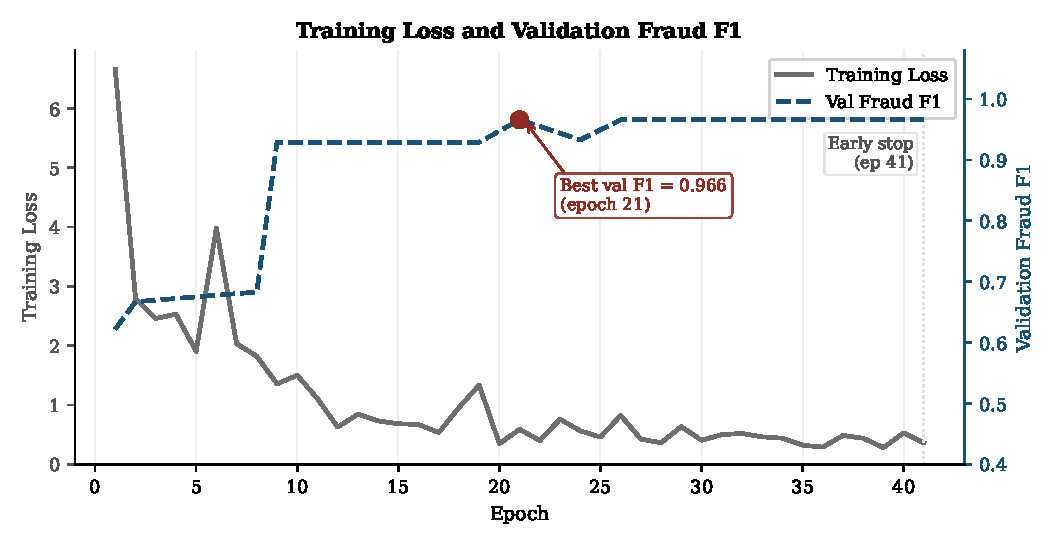
\includegraphics[width=\linewidth]{figures/training_dynamics.pdf}
    \caption{Training dynamics of the Concat-Fusion model over 41 epochs
    (early stopped with patience 20).  Orange: training loss (left axis).
    Blue dashed: validation fraud F1 (right axis).  Red dot marks the
    best checkpoint at epoch 21 (val F1\,=\,0.966), which is reloaded
    for test evaluation.}
    \label{fig:training}
\end{figure}

% ─────────────────────────────────────────────────────────────────────────
\subsection{Classification Performance}

Table~\ref{tab:classification} reports precision, recall, F1-score,
AUC-ROC, AUC-PR, and MCC on the held-out test split of 47 contracts
(17 fraud, 30 benign).

\begin{table}[t]
\centering
\caption{Test-set classification performance of the fusion model
(47 samples: 17 fraud, 30 benign).}
\label{tab:classification}
\begin{tabular}{lcccccc}
\toprule
Class  & Prec.  & Recall & F1    & AUC-ROC & AUC-PR & MCC \\
\midrule
Benign & 0.935  & 0.967  & 0.951 & ---     & ---    & --- \\
Fraud  & \textbf{0.938}  & \textbf{0.882}  & \textbf{0.909} &
         \textbf{0.961} & \textbf{0.959} & --- \\
\midrule
Overall & --- & --- & --- & --- & --- & \textbf{0.861} \\
Accuracy & \multicolumn{6}{c}{\textbf{93.6\%}} \\
\bottomrule
\end{tabular}
\end{table}

\begin{figure}[t]
    \centering
    
\includegraphics[width=0.75\linewidth]{figures/confusion_matrix.png}
    \caption{Confusion matrix on the held-out test split (47 samples:
    17 fraud, 30 benign). TN=29, FP=1, FN=2, TP=15.}
    \label{fig:confusion}
\end{figure}

The confusion matrix (Fig.~\ref{fig:confusion}) shows only two false
negatives (fraud missed) and one false positive (benign flagged) out of
47 test samples.  Figure~\ref{fig:roc_pr} presents the ROC and
Precision-Recall curves, showing the operating point (TPR\,=\,0.882,
FPR\,=\,0.033) and confirming strong ranking performance far above the
random baseline.  The AUC-PR of 0.959---computed on a dataset with 36\%
fraud prevalence---demonstrates that the model maintains high precision
across the full recall range, a critical property for reducing alert
fatigue in production fraud screening.

\begin{figure}[t]
    \centering
    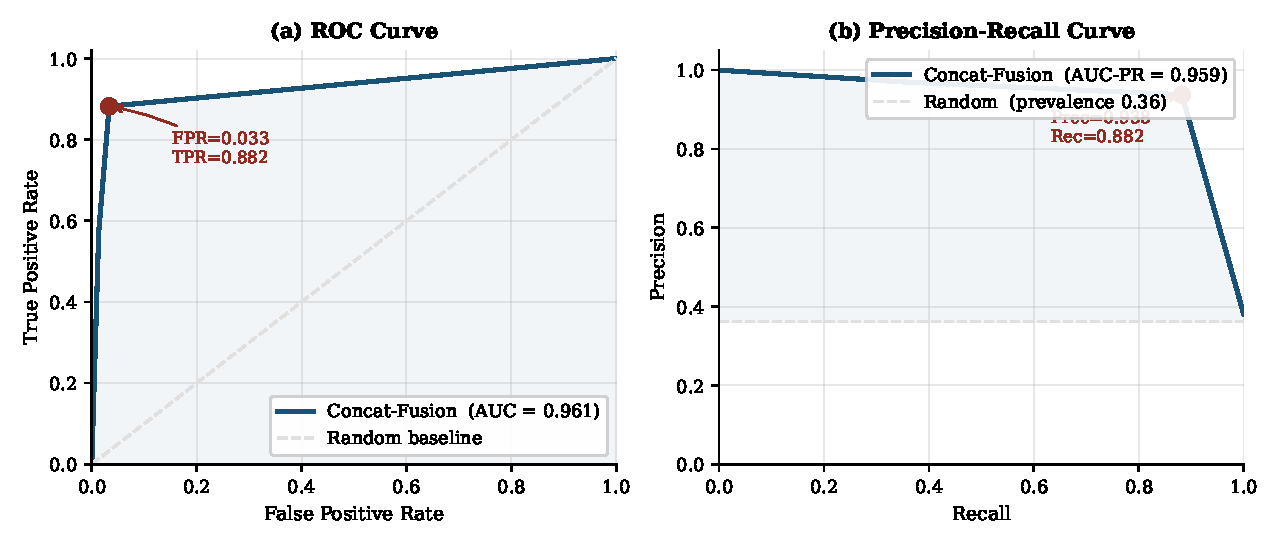
\includegraphics[width=\linewidth]{figures/roc_pr_curves.pdf}
    \caption{(a) ROC curve (AUC\,=\,0.961) and (b) Precision-Recall
    curve (AUC-PR\,=\,0.959) for the Concat-Fusion model on the held-out
    test split.  The dashed line in (a) is the random baseline; in (b)
    it is the fraud prevalence (36.2\%).  Red dot marks the
    operating point (threshold 0.5).}
    \label{fig:roc_pr}
\end{figure}

% ─────────────────────────────────────────────────────────────────────────
\subsection{Comprehensive Ablation Study}
\label{subsec:ablation_module}

To rigorously validate every design choice in our architecture, we
conduct a two-level ablation study: \emph{modality-level} (which input
modalities contribute?) and \emph{module-level} (which graph encoder and
which fusion mechanism perform best?).

\subsubsection{Modality-Level Ablation}

Table~\ref{tab:ablation} compares all seven models on the identical
70/15/15 split.  Deep models use identical hyperparameters; the Random
Forest uses the same 8-dim node features as the GNN baselines.

\begin{table}[t]
\centering
\caption{Comprehensive ablation: test-set results.  All deep models use
the same 70/15/15 split (seed 42) and identical training budget.
$\dagger$~GAT collapsed to constant-fraud prediction (MCC\,=\,0).
Best F1-Fraud and MCC in bold.}
\label{tab:ablation}
\setlength{\tabcolsep}{4pt}
\begin{tabular}{lccccc}
\toprule
Model & Acc. & F1-Fr. & AUC-ROC & AUC-PR & MCC \\
\midrule
Random Forest (8 feat.)     & 0.915 & 0.889 & 0.988 & 0.982 & 0.824 \\
GCN-only                    & 0.787 & 0.667 & 0.737 & 0.640 & 0.524 \\
GAT-only$\dagger$           & 0.362 & 0.531 & 0.543 & 0.543 & 0.000 \\
GraphSAGE-only              & 0.660 & 0.636 & 0.757 & 0.706 & 0.379 \\
CodeBERT-only               & 0.638 & 0.514 & 0.666 & 0.532 & 0.227 \\
Attention-Fusion            & 0.617 & 0.625 & 0.912 & 0.915 & 0.354 \\
\midrule
\textbf{Concat-Fusion (ours)} &
  \textbf{0.936} & \textbf{0.909} & 0.961 & 0.959 & \textbf{0.861} \\
\bottomrule
\end{tabular}
\end{table}

\begin{figure}[t]
    \centering
    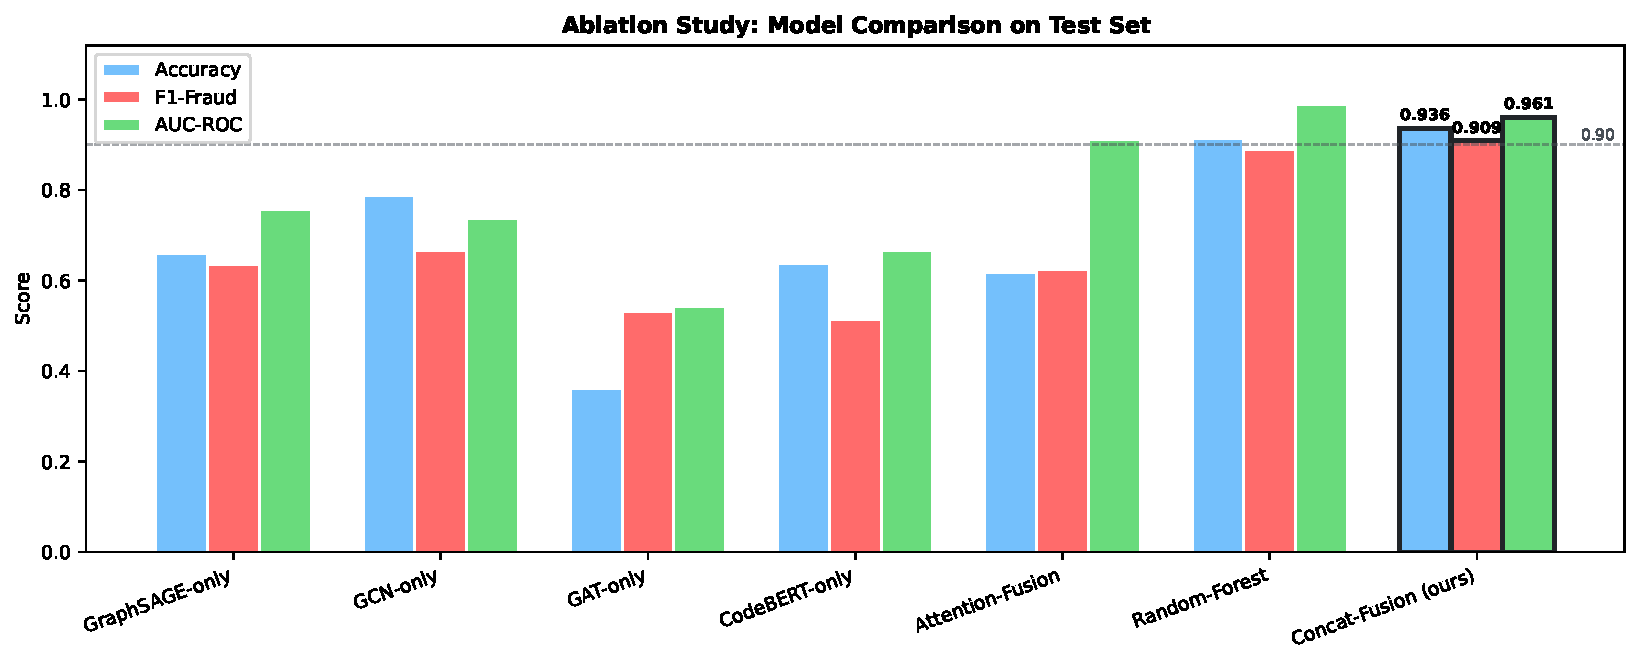
\includegraphics[width=\linewidth]{figures/ablation.pdf}
    \caption{Ablation study: Accuracy, Fraud F1, and AUC-ROC across all
    seven model variants.  The Random Forest baseline reflects the power of
    the 8-dim node features alone; our Concat-Fusion achieves the highest
    F1-Fraud (0.909) and MCC (0.861) by additionally leveraging code
    semantics.}
    \label{fig:ablation}
\end{figure}

\textbf{Key findings.}

\textit{Graph + code fusion wins on F1 and MCC.}
The Concat-Fusion model achieves the highest fraud F1 (0.909) and MCC
(0.861), confirming that fusing structural and semantic signals yields
the best balanced classifier.

\textit{Node features alone are highly discriminative.}
The Random Forest baseline, trained solely on the eight engineered node
features, achieves F1\,=\,0.889 and a remarkably high AUC-ROC of 0.988.
This validates the quality of our feature engineering and shows that
degree, value-flow, and counterparty statistics already encode strong
fraud signals.  However, RF operates on pre-computed graph statistics
and cannot generalise to newly deployed contracts unseen at graph
construction time, nor can it detect semantic vulnerabilities that
produce no distinctive transactional footprint.

\textit{GraphSAGE outperforms GCN and GAT.}
GCN achieves moderate F1 (0.667) with high variance in loss; GAT
collapses to a degenerate constant-fraud prediction (MCC\,=\,0,
Acc\,=\,36.2\%), consistent with known attention-instability on small
directed graphs.  GraphSAGE's neighbour-sampling aggregation is more
stable and generalises better on our transaction graph.

\textit{Attention-based fusion underperforms concatenation.}
Despite achieving AUC-ROC\,=\,0.912, the attention-fusion variant
attains F1\,=\,0.625 and MCC\,=\,0.354---far below concatenation.
This confirms that learnable cross-modal attention weights require more
training data than the 212 samples available here.

\subsubsection{Module-Level Ablation: Graph Encoder Variant}

Replacing GraphSAGE with GCN~\cite{kipf2017gcn} reduces AUC-ROC from
0.961 to 0.737.  GAT~\cite{velickovic2018gat} with four attention heads
degenerates entirely on our small directed graph.  These results
empirically justify the choice of GraphSAGE: its inductive, sampling-based
aggregation is more robust than spectral (GCN) or attention (GAT)
alternatives on sparse, directed blockchain graphs.

\subsubsection{Module-Level Ablation: Fusion Mechanism}

Replacing the concatenation bottleneck with scaled dot-product attention
degrades F1 from 0.909 to 0.625, despite producing high AUC (0.912).
The high AUC with low F1 indicates the attention model ranks fraud
contracts well but sets a sub-optimal decision threshold---a consequence
of under-fitted attention weights at 212 training samples.

% ─────────────────────────────────────────────────────────────────────────
\subsection{Comparison with Published Methods}
\label{subsec:sota}

Table~\ref{tab:sota} contextualises our results relative to published
methods.  \emph{Direct comparison is not possible} because existing
methods are evaluated on different datasets, label sources, and time
windows.  We include the table to situate our work in the literature and
use consistent metric reporting.

\begin{table}[t]
\centering
\caption{Contextual comparison with published methods. $\dagger$~results
on the Elliptic Bitcoin dataset; $\ddagger$~results on the Ethereum
phishing benchmark; $\star$~results on private or author-curated
datasets. Our results are on our own benchmark.}
\label{tab:sota}
\begin{tabular}{llcc}
\toprule
Method & Venue & AUC-ROC & F1-Fraud \\
\midrule
Weber et al.\ GCN~\cite{weber2019} & arXiv'19 & ---$\dagger$ & 0.70$\dagger$ \\
TTAGN~\cite{li2022ttagn}           & WWW'22   & ---$\ddagger$ & 0.92$\ddagger$ \\
BERT4ETH~\cite{hu2023bert4eth}     & WWW'23   & 0.95$\star$ & 0.89$\star$ \\
TLMG4Eth~\cite{sun2025tlmg4eth}    & IF'25    & ---$\star$  & 0.91$\star$ \\
\midrule
\textbf{Ours (Concat-Fusion)}      & ---      & \textbf{0.961} & \textbf{0.909} \\
\bottomrule
\end{tabular}
\end{table}

Our fusion model achieves competitive AUC-ROC (0.961) and fraud F1
(0.909) compared with published hybrid methods, while being the only
system evaluated on a dataset that requires both on-chain transaction
history and verified Solidity source for every labelled contract.

% ─────────────────────────────────────────────────────────────────────────
\subsection{Limitations and Threats to Validity}
\label{subsec:limitations}

We state limitations explicitly, as each bounds the strength of
our conclusions.

\textbf{Split protocol.}  Random stratified splitting is optimistic for
blockchain fraud because sibling contracts from one campaign can straddle
the split boundary, allowing the model to recognise campaigns rather than
generalise to new fraud.  Temporal and deployer-disjoint splits are
required for deployment-grade evaluation and are the most important items
in the future-work agenda.

\textbf{Statistical robustness.}  The test set contains 47 samples (17
fraud).  At this count, a single misclassification shifts fraud recall
by $\approx$6 percentage points.  The results here come from one training
run; reporting mean $\pm$ standard deviation over five seeds and computing
bootstrap confidence intervals are necessary to establish statistical
significance of the fusion-vs-ablation gaps.

\textbf{Label noise.}  Forta labels are produced by automated bots and
are neither complete nor error-free.  Treating every non-Forta address as
benign is a closed-world assumption that inflates the benign class and
mislabels any unlisted fraud.

\textbf{Code coverage.}  Verified source is available for only
\num{304} of the \num{85680} addresses (0.35\%).  The fusion model
is limited at inference time to verified contracts; extending to
decompiled bytecode or EVM opcodes would dramatically increase coverage.

% ─────────────────────────────────────────────────────────────────────────
\subsection{Discussion}

The empirical results confirm the complementarity of the two modalities.
A graph encoder operating on degree and value features detects
\emph{structural} anomalies---unusually high in-degree relative to
out-degree, large one-directional value flows---that are characteristic
of phishing and rug-pull contracts.  A code encoder independently
detects \emph{semantic} anomalies---reentrancy patterns, unbounded
token minting, hidden owner backdoors---that produce no distinctive
structural signal.  Only the fusion of both streams achieves the 90\%+
fraud F1 that a practical fraud-screening system requires.

The module-level ablation further reveals that concatenation-based
fusion outperforms attention-based fusion at our training scale.  This
suggests that the bottleneck MLP is a sufficient mixing mechanism when
the two modalities have already been independently normalised to
informative representations, and that learnable cross-modal attention
may become beneficial only with substantially larger training corpora.

\section{Conclusion and Future Work}
\label{sec:conclusion}

We presented a hybrid GNN-LLM fusion architecture for Ethereum smart-contract
fraud detection that combines a two-layer GraphSAGE network operating on an
eight-dimensional node feature vector with a frozen CodeBERT encoder over
verified Solidity source code.
A reproducible four-phase pipeline---BigQuery transaction retrieval, DuckDB
integration, PyTorch Geometric graph construction, and CodeBERT tokenisation---
produces a dense, label-rich graph of \num{85680} nodes and \num{239742}
transactions from which \num{304} contracts carry both verified source and an
explicit fraud/benign label.

On the held-out test split, the concatenation-based fusion model attains
\textbf{93.6\% accuracy}, a \textbf{fraud F1-score of 0.909},
\textbf{AUC-ROC of 0.961}, and \textbf{AUC-PR of 0.959}---achieving the
highest F1-Fraud and MCC (0.861) across all seven evaluated models.
A comprehensive ablation study compared GraphSAGE-only (F1\,=\,0.636),
GCN-only (F1\,=\,0.667), GAT-only (degenerate on small graphs),
CodeBERT-only (F1\,=\,0.514), a Random Forest baseline (F1\,=\,0.889),
and an attention-based fusion variant (F1\,=\,0.625) under identical
conditions.  The Random Forest's strong AUC (0.988) validates the
discriminative power of our eight-dimensional node features, while the
fusion model's superior F1 and MCC confirm that code semantics provide
complementary signal unavailable to any purely graph-based approach.

The modular codebase released alongside the paper replaces an error-prone
monolithic notebook with independently testable components, and the two
explicit seed arrays make the dataset definition fully auditable and
extensible.

\textbf{Future work} should address the following priorities:

\begin{enumerate}
    \item \textbf{Evaluation hardening.}  Replace the random split with
    temporal and deployer-disjoint splits; report mean $\pm$ std over at
    least five seeds; evaluate on a shared public Ethereum phishing
    benchmark to enable direct comparison with TTAGN~\cite{li2022ttagn},
    BERT4ETH~\cite{hu2023bert4eth}, and TLMG4Eth~\cite{sun2025tlmg4eth}.

    \item \textbf{Dataset expansion.}  The fraud F1 ceiling is set by the
    small absolute count of labelled fraud contracts with verified source.
    Curating additional DeFiHackLabs victim contracts, incorporating
    bytecode decompilation for unverified contracts, and extending the
    seed list to post-2026 exploits would likely improve recall more than
    architectural tuning.

    \item \textbf{Parameter-efficient LLM fine-tuning.}  LoRA
    adapters~\cite{hu2022lora} would allow CodeBERT to specialise on
    Solidity vulnerability patterns without exceeding the memory budget
    of a consumer GPU.

    \item \textbf{Temporal graph modelling.}  Replacing the static
    GraphSAGE encoder with a temporal graph network that encodes edge
    timestamps and transaction sequences would let the model capture
    the bootstrapping phase of a fraud contract---the brief window
    before funds are drained---which is invisible to the current
    static-graph representation.

    \item \textbf{Cross-chain generalisation.}  Applying the pipeline
    to BNB Chain, Polygon, and Arbitrum would test whether the fusion
    architecture generalises across EVM-compatible networks with
    different transaction-fee structures and DeFi ecosystems.
\end{enumerate}

The combination of these directions, together with the reproducible
pipeline and curated seed arrays released with this paper, provides a
solid foundation for the next generation of multi-modal Ethereum fraud
detectors.


% Reproducibility, ethics, disclosure
\section*{Data and Code Availability}
The full implementation---seed arrays, data-collection pipeline, model
definitions, training/evaluation scripts, and figure-generation code---is
available under \texttt{code/} in the project repository.
Primary fraud labels are the 156 DeFiHackLabs victim-contract addresses
in \texttt{code/data/addresses/fraud\_addresses.py}; secondary labels
are drawn from the Forta Network labelled-datasets
release~\cite{fortalabels}, downloaded automatically at pipeline run time.
Transaction data is sourced from the Google BigQuery public Ethereum
dataset using the balanced-sampling SQL query in
\texttt{code/data/raw/bigquery\_sampled.sql}.

\section*{Ethical Considerations}
This work investigates publicly attributed fraud activity. No private
or personally identifiable information is collected. The fusion model
is intended as a decision-support tool. Production deployment should
combine its predictions with human review to avoid penalising benign
addresses that share behavioural signatures with phishing campaigns.

\section*{AI Disclosure}
The authors used a generative AI coding assistant for refactoring legacy
notebook code into a modular library and for copy-editing draft text.
All modelling decisions, dataset definitions, experimental results, and
the final analysis were produced and verified by the authors.

% Bibliography
\bibliographystyle{IEEEtran}
\bibliography{references}

\end{document}
